% \documentclass{beamer}
% \usepackage{subcaption} 
% \usepackage{array}
% \usepackage{booktabs}
% \usepackage{wasysym}
\providecommand{\ex}[1]{\ensuremath{^{#1}}}
\newcommand{\msun}{M_\odot}
\newcommand{\element}[2]{^{#1}\text{#2}}
\newcommand{\iso}[2]{$^{#1}${#2}}

\documentclass[10pt]{beamer}
\usetheme[progressbar=frametitle]{metropolis}
\usepackage{appendixnumberbeamer}
\usepackage{cutwin}
\usepackage{lipsum}
\usepackage[3D]{movie15}
\usepackage[dutch]{babel}

\usepackage{booktabs}
\usepackage[scale=2]{ccicons}
\usepackage{subcaption} 
\usepackage[font=scriptsize]{caption}
\usepackage{pgfplots}
\usepgfplotslibrary{dateplot}

\usepackage{xspace}
\newcommand{\themename}{\textbf{\textsc{metropolis}}\xspace}
\usepackage{wasysym}

\setbeamersize{text margin left=5mm,text margin right=5mm} 
\usepackage[round]{natbib}
\bibliographystyle{aasjournal}



\title{The Impact of Nuclear Uncertainties on the GCE of Si Isotopes}
\date{}

\author{\textbf{Hung Kwan Fok}}
\institute{Brandeis University}


\begin{document}

\maketitle
% \begin{frame}{Outline}
%     \begin{itemize}
%     \setlength\itemsep{2em}
%         \item Introduction
%         \begin{itemize}
%             \item Galactic chemical evolution (GCE)
%             \item Stardust grains and Mainstream grains
%         \end{itemize}

%         \item Methods and Goals
%         \begin{itemize}
%             \item Monte Carlo
%         \end{itemize}

%         \item Results

%     \end{itemize}
    
% \end{frame}

\begin{frame}{Galactic Chemical Evolution (GCE)}

\begin{minipage}{5.5cm}
    \begin{itemize}
    \setlength\itemsep{2em}
        \item GCE describes the evolution of elements since the Big Bang
        \item Elements heavier than Li are produced in stars and recycled back into the galaxy when they die
        \item Metallicity Z: mass fraction of elements heavier than helium 
    \end{itemize}
\end{minipage}
\hspace*{3mm}
\begin{minipage}{4.5cm}
    \begin{figure}
        \centering
        \includegraphics[width=\textwidth]{figs/Crab_Nebula.jpg}
        \caption*{Credit: NASA, ESA, J. Hester and A. Loll (Arizona State University)}
    \end{figure}
\end{minipage}
    
\end{frame}
% GCE describes the evolution of elements since the big bang. Essentially, it is a story about where everything we see around us comes from by tracing all the way back to the big bang. A short version of this story is that all the stars formed since the big bang synthesis the chemical elements in them and recycled the elements back to the galaxy when they died. so how do we trace the story of GCE? stardust

\begin{frame}{Stardust Grains}
    \begin{minipage}{5cm}
    \begin{itemize}
        \setlength\itemsep{1em}
        \item Formed in the outflow of dying stars
        \item Can be found and recovered from meteorites
        \item Allow for high precision measurements of isotopic compositions
        \item Useful in constraining stellar nucleosynthesis and GCE models
    \end{itemize}
    \end{minipage}
    \hspace*{3mm}
    \begin{minipage}{6.1cm}

        \begin{figure}
            \centering
            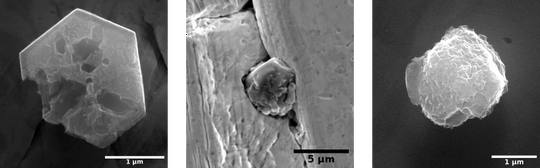
\includegraphics[width=\textwidth]{figs/stardust.png}
        \end{figure}
    \end{minipage}
    
    %%%%%%
    % stardust grains are formed in the outflow of dying stars and subsequently mixed into the ISM. These grains are interesting because they carry the nucleosynthesis signature of their parent star and we can make high precision measurements of the isotopic composition of the stardust grains. These information is useful in constraining the models of stellar nucleosynthesis and GCE.
\end{frame}

\begin{frame}{Origin of Stardust Grains}
    \begin{figure}
        \centering
        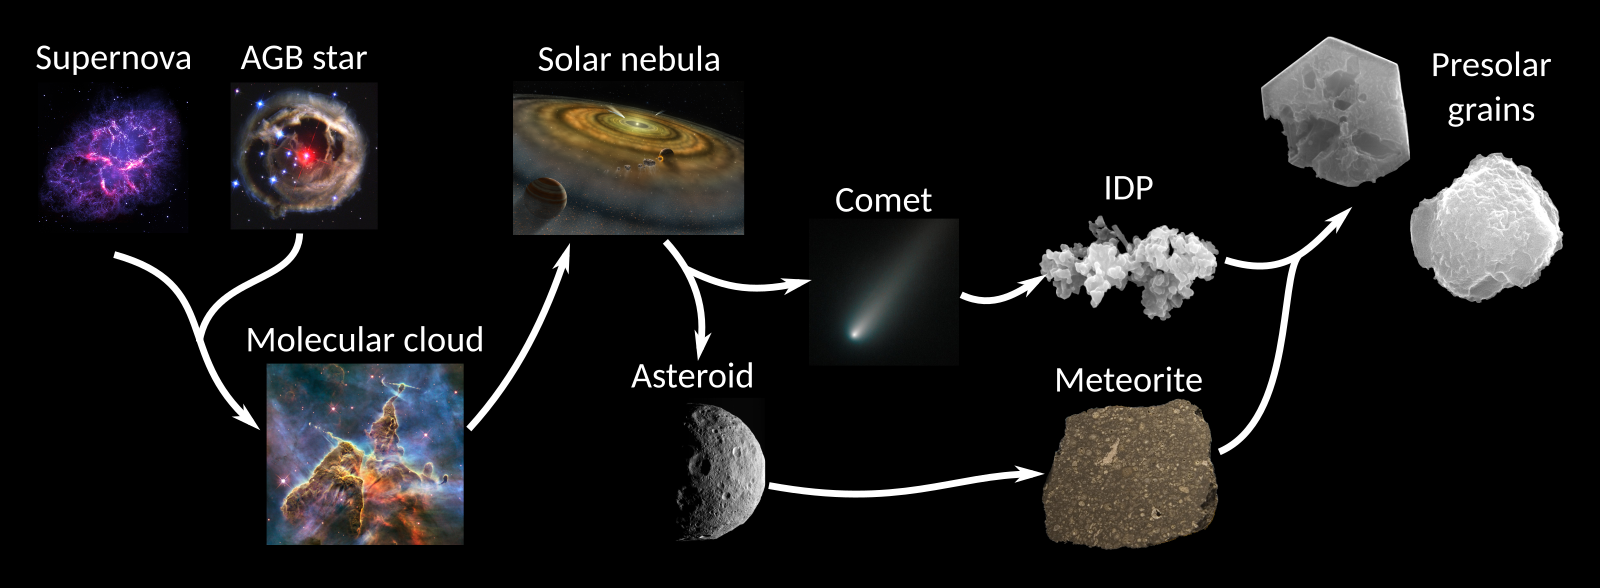
\includegraphics[scale = 0.2]{figs/presolar_grains_origin_1600.png}

    \end{figure}
    
    %%%%%%
    % Here shows the whole history of stardust grains. some of these particles will become part of the molecular cloud from which the solar system is formed. During the formation of solid in the solar system, stardust grains are incorporated into meteorite parent bodies and can be found in the primitive meteorite.
    
\end{frame}


\begin{frame}{Mainstream Grains Contain GCE Signature}
    \begin{minipage}{5cm}
    \begin{itemize}
    \setlength\itemsep{2em}
        \item Mainstream grains from AGB stars
        
        \item The Si isotopic composition of mainstream grains is a GCE signature
        
        % \item Cannot be explained by the current GCE models

        \item $\delta-$unit: deviation from solar
        
        % : show the plots of omega runs with different stellar yields comparing with mainstream grains
    \end{itemize}
    \end{minipage}
    \begin{minipage}{6.6cm}
        \begin{figure}
            \centering
            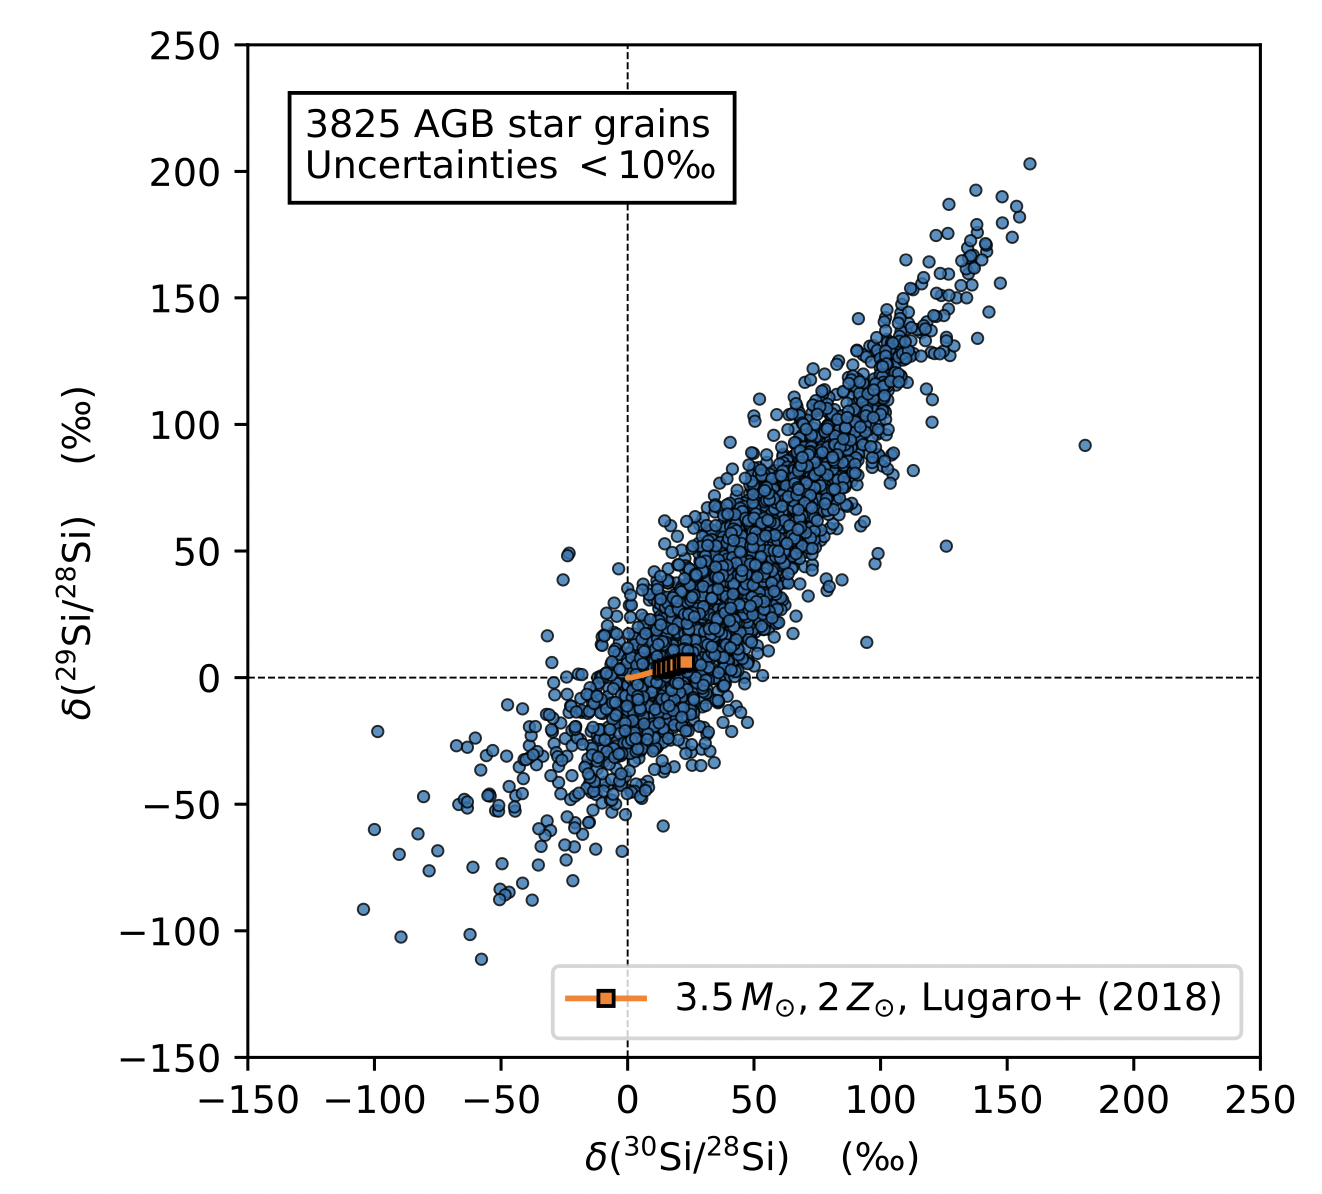
\includegraphics[width = \textwidth]{figs/agb.png}
        \end{figure}
    \end{minipage}
    
    %%%%%%%
    % focusing on the silicon isotopic composition in mainstream grain because they are believed to contains GCE signature. 
    % The orange line: represents the whole evolution of AGB stars. we can see that they cannot explain the distribution we found in mainstream grain. So this means that although the mainstream grains are produced in AGB stars,  Nucleosynthesis in AGB stars cannot explain their silicon isotopic composition. 
\end{frame}


\begin{frame}{GCE Models Cannot Explain Silicon Isotopes Analysed in Mainstream Grains}
    \begin{minipage}{4.5cm}
    
    Two main issues:\\


    \begin{itemize}
    \setlength\itemsep{2em}
        \item Enriched with \iso{29,\, 30}{Si} elements compared to Solar System
        \begin{itemize}
            \item Heterogeneous GCE 
        \end{itemize}
        \item \alert{The slope of the correlation line}

        
        % : show the plots of omega runs with different stellar yields comparing with mainstream grains
    \end{itemize}
    \end{minipage}
    \begin{minipage}{7cm}
        \begin{figure}
            \centering
            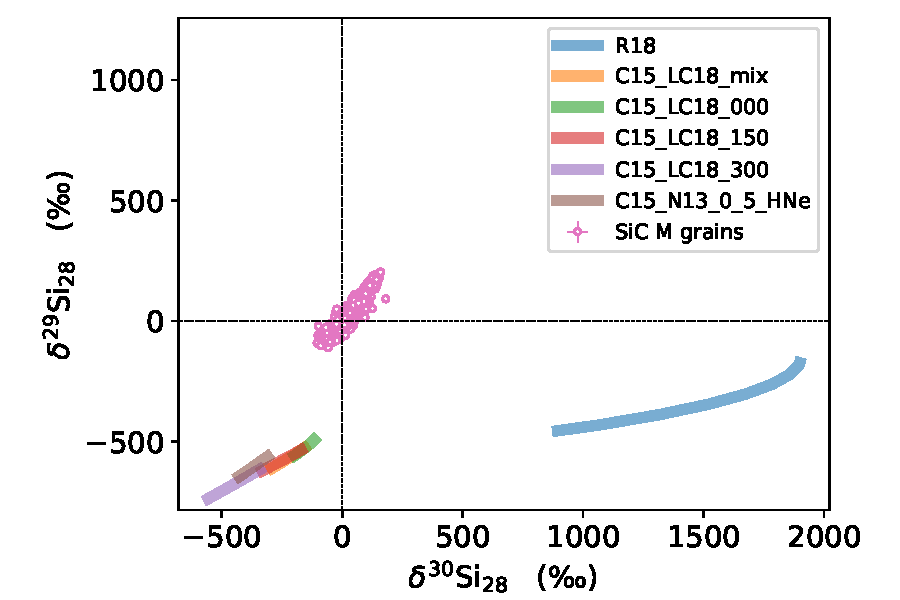
\includegraphics[width=\textwidth]{figs/gce_Si_isotope.pdf}
            
        \end{figure}
    \end{minipage}
    
    %%%%%%%%
    % However, the silicon isotopic composition in mainstream grains cannot be explained by the current gce model. the plot here shows the comparison between the mainstream grains data with different GCE simulations. There are two main issues: 1) the mainstream grains are enriched with secondary elements (silicon 29, 30) compared to solar system. One approach to explain it is the heterogeneous gce model. 2) the slope of the silicon isotope ratio correlation line. In particular, the slope measured in the grains is larger than the slope calculated from the gce model. 
\end{frame}

\begin{frame}{Can Nuclear Reaction Rate Uncertainties Explain this Slope?}
    \begin{itemize}
    \setlength\itemsep{2em}
        \item Focus on nuclear uncertainties in stellar nucleosynthesis 
        % \begin{itemize}
        %     \item \cite{Timmes_1996}: ``changes to the nuclear reaction rates may be the most appropriate answer [to increase $\element{29}{Si}/\element{30}{Si}$ ratio]"
        %     \item \cite{Hoppe_2009}: calculated $\element{29}{Si}/\element{28}{Si}$ ratio match with the value measured in a grain that originated from a supernova by increasing $\element{26}{Mg} (\alpha, n) \element{29}{Si}$ by a factor of 3 
        % \end{itemize}
    \end{itemize}
    \textbf{Our goal:}
    \begin{itemize}
    \setlength\itemsep{2em}
        \item Identify the stars that are responsible for silicon production
        \item Identify the main Si-production regions in those stars and the relevant reaction rates
        \item Monte Carlo Framework:
        \begin{itemize}
            \item Calculate the nucleosynthesis in the relevant regions and the resulting stellar yield with varying reaction rates
            \item Calculate the GCE of Si isotopes using the modified stellar yields
        \end{itemize}
        
    \end{itemize}
    
    %%%%%%%%
    % so we propose this question that we are trying to answer in this project: will... . multiple works have indicate such possibility but no one have tried. 
\end{frame}


\begin{frame}{Massive Stars are the Main Source of Silicon in the Galaxy}
     Focus on stellar models with initial mass $M/\msun = 15, 20$ at metallicity $Z=0.02, 0.01$

    \begin{figure}
        \begin{subfigure}[b]{0.48\textwidth}
            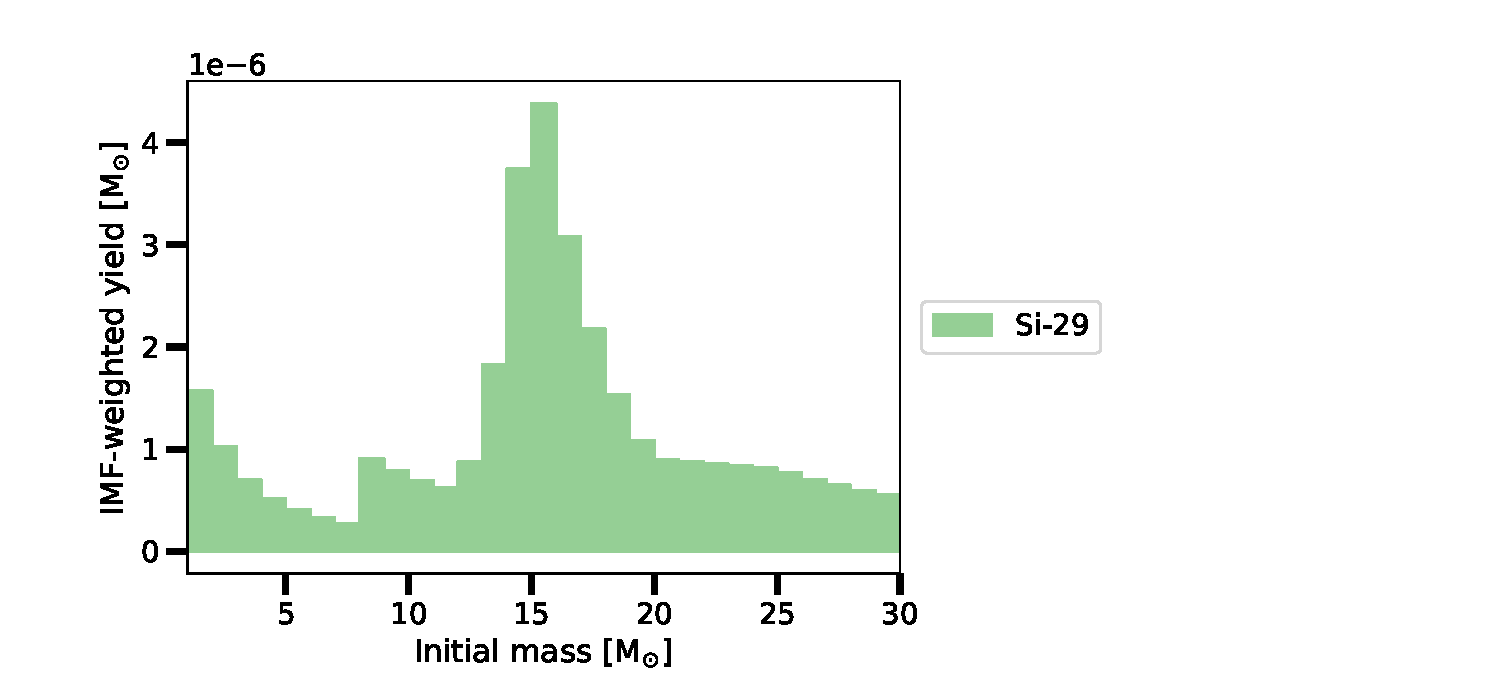
\includegraphics[width=\textwidth]{figs/Si-29_Z=0.01_yield.pdf}
        \end{subfigure}
        \begin{subfigure}[b]{0.48\textwidth}
            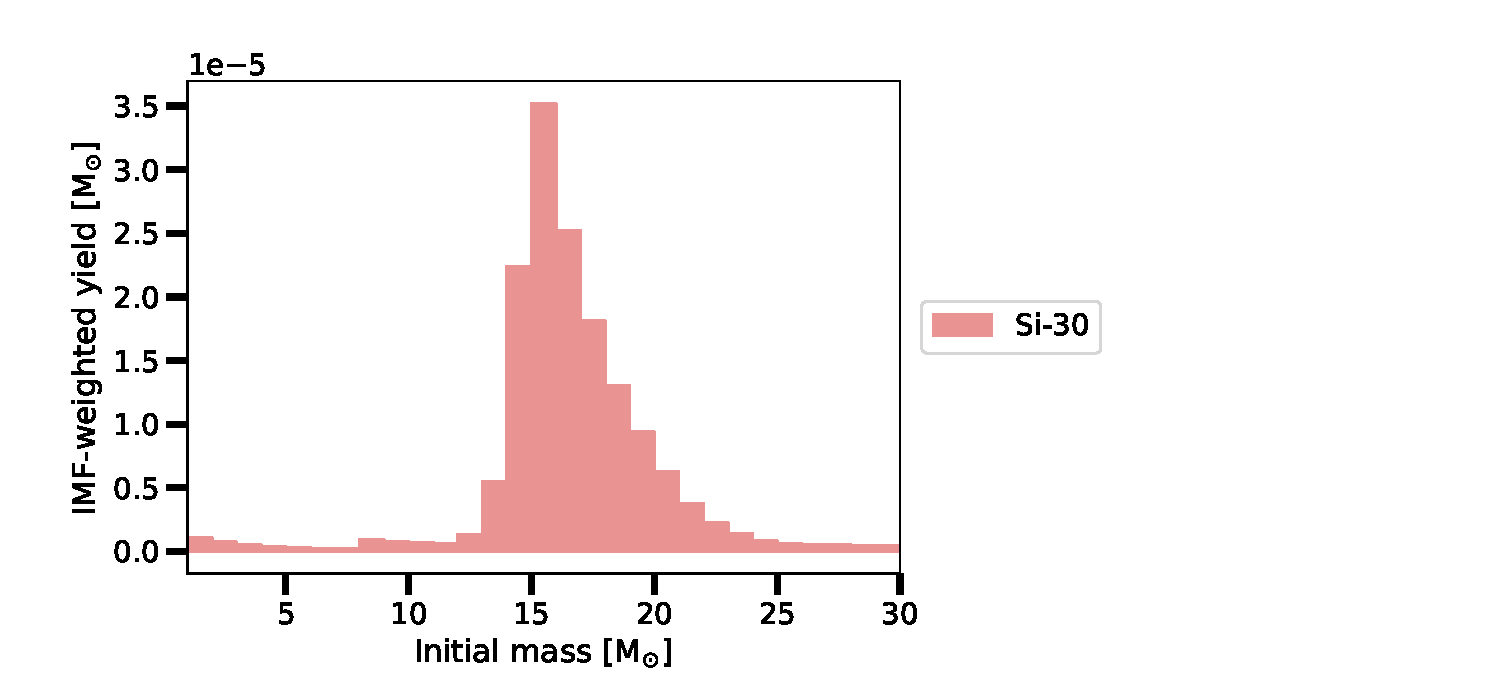
\includegraphics[width=\textwidth]{figs/Si-30_Z=0.01_yield.pdf}
        \end{subfigure}
        \begin{subfigure}[b]{0.48\textwidth}
            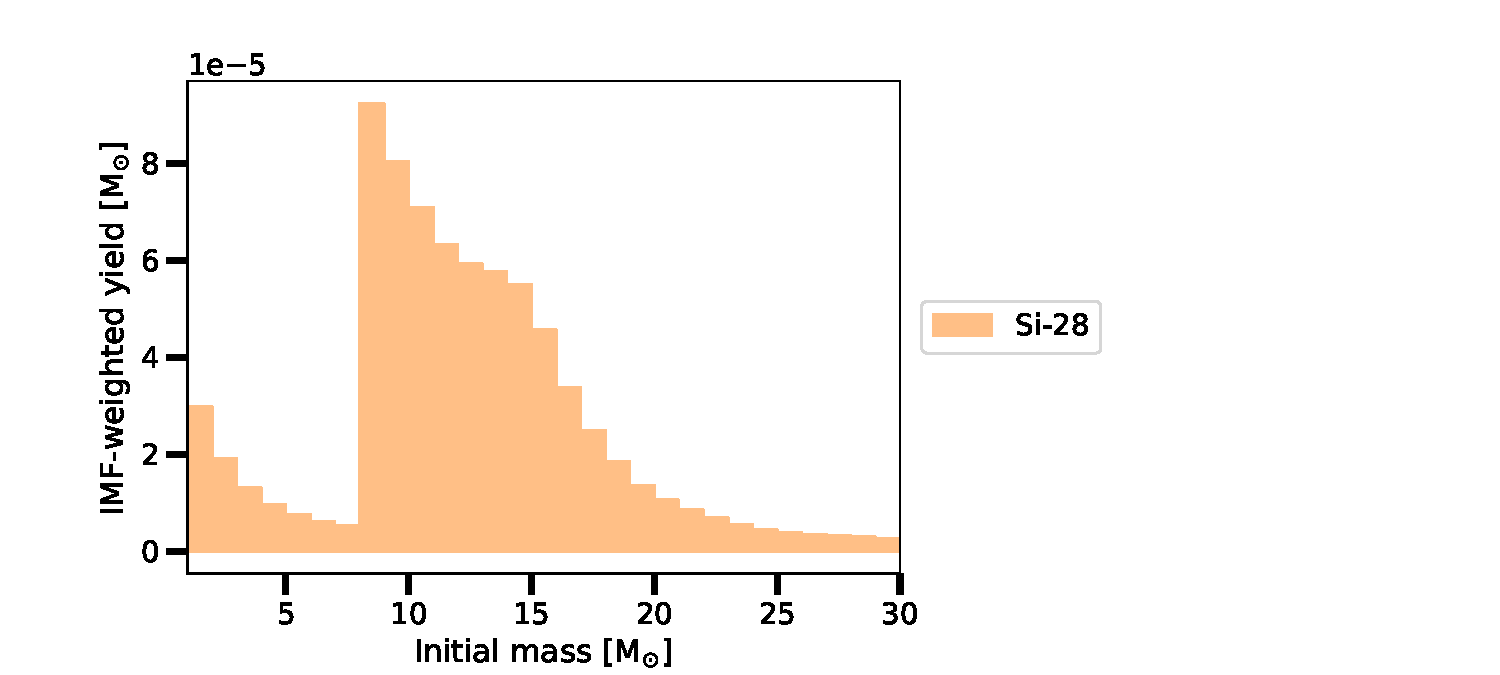
\includegraphics[width=\textwidth]{figs/Si-28_Z=0.01_yield.pdf}
        \end{subfigure}
    \end{figure}
    % first question we want to answer is what are the stars that are responsible for the production of silicon in the galaxy. here shows the imf weighted silicon yields for different initial masses. from the plot we can see that the massive stars are the main producer of silicon. massive star refers to stars with initial mass greater than 12 solar mass. 
    %%%%%%%%%
    % so why we are focusing on nucleosynthesis in massive stars: here's some evidences from the imf weighted silicon yields for different initial masses. shown here is the stars with 0.02 metalicity. from the plot we can see that the massive stars are the main producer of silicon
\end{frame}



\begin{frame}{Silicon Produced in Explosive Oxygen Burning}
    \begin{minipage}{5cm}
        \begin{itemize}
        \setlength\itemsep{2em}
            \item Focus on explosive nucleosynthesis
            \item Here: Compare the pre-supernova composition with final composition
            % \item Silicon isotopes are produced during explosive oxygen burning
        \end{itemize}
    \end{minipage}
    \begin{minipage}{6.5cm}
    \centering
        \begin{figure}
            \centering
            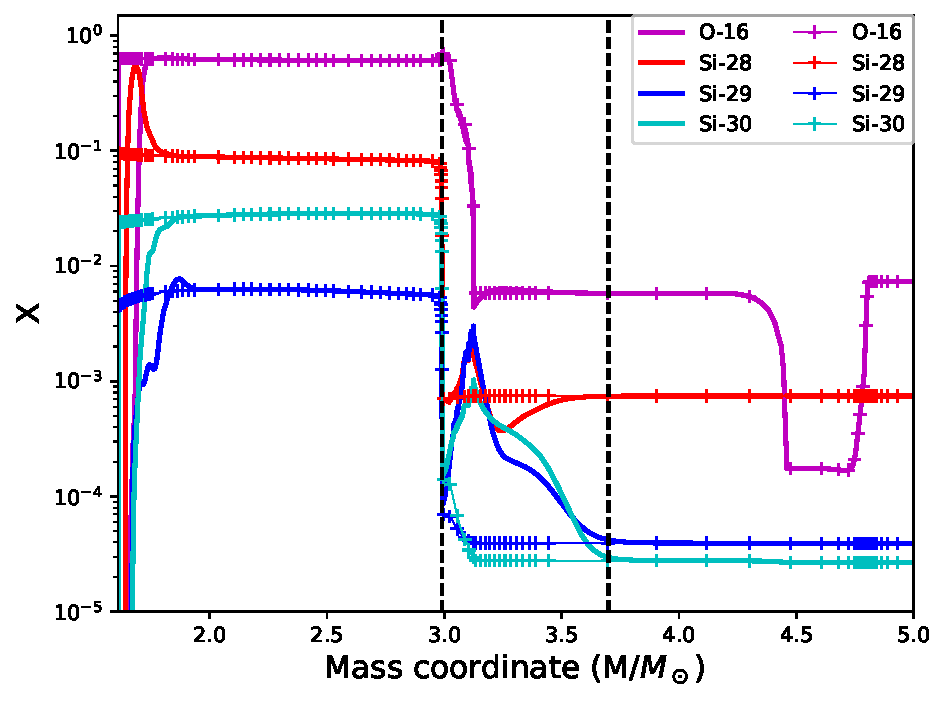
\includegraphics[width = \textwidth]{figs/explosive.pdf}
        \end{figure}
    \end{minipage}   
\end{frame}
% we then move on to the next question of where in the star is silicon produced. heavy silicon isotopes are formed during the ccsn explosion of massive stars. in particular, in the explosive oxygen burning region. 


\begin{frame}{Silicon Production Reactions}
    \begin{minipage}{5cm}
        \begin{itemize}
        \setlength\itemsep{2em}
            \item The upper and lower limits of the $(n, \gamma)$ reactions are based on experimental errors.
            \item The limit of other reactions are based on theoretical limits given by \cite{Rauscher_2016}.
        \end{itemize}
    \end{minipage}
    \begin{minipage}{6.5cm}
\begin{table}[H]
    \centering
    \caption{Main silicon production/destruction reaction rates and the upper ($U^{\rm hi}$) and lower ($U^{\rm lo}$) limits of their variation factors.}
\begin{tabular}{c c c}
    \hline
      Reaction  & $U^{\rm hi}$ & $U^{\rm lo}$\\
    \hline
    \iso{28}{Si}$(n, \gamma)$\iso{29}{Si}& 1.18 & 0.82\\
    \iso{29}{Si}$(n, \gamma)$\iso{30}{Si}& 1.20 & 0.80\\
    \iso{30}{Si}$(n, \gamma)$\iso{31}{Si}& 1.36 & 0.64\\
    \iso{25}{Mg}$(\alpha, n)$\iso{28}{Si}& 2.00 & 0.10\\
    \iso{26}{Mg}$(\alpha, n)$\iso{29}{Si}& 2.00 & 0.10\\
    \iso{33}{S}$(n, \alpha)$\iso{30}{Si}& 2.00 & 0.10\\
    \hline
    \end{tabular}
    \label{tab:si_reaction}
\end{table}
    \end{minipage}
    
    % in the silicon production regions, we identified six nuclear reactions that are most important for silicon production and destruction. the table shows the upper and lower limits of the rate variation factors we used in our monte carlo simulations. for example, n gamma on si28 is varied between 1.18 and 0.82 times the default rate. 
    
\end{frame}

\begin{frame}{Nuclear Uncertainties Affect Nucleosynthesis of Silicon in Stars}
    \begin{minipage}{5cm}
        \begin{itemize}
            \setlength\itemsep{2em}
            \item \iso{29,\, 30}{Si} abundances are affected by nuclear uncertainties
            \item \iso{28}{Si} abundances remain largely unchanged
            % \item Up to 73\% increase in \iso{29}{Si} abundances
            % \item Up to 45\% increase in \iso{30}{Si} abundances
        \end{itemize}
    \end{minipage}
    \begin{minipage}{6.5cm}
    \centering
        \begin{figure}
            \centering
            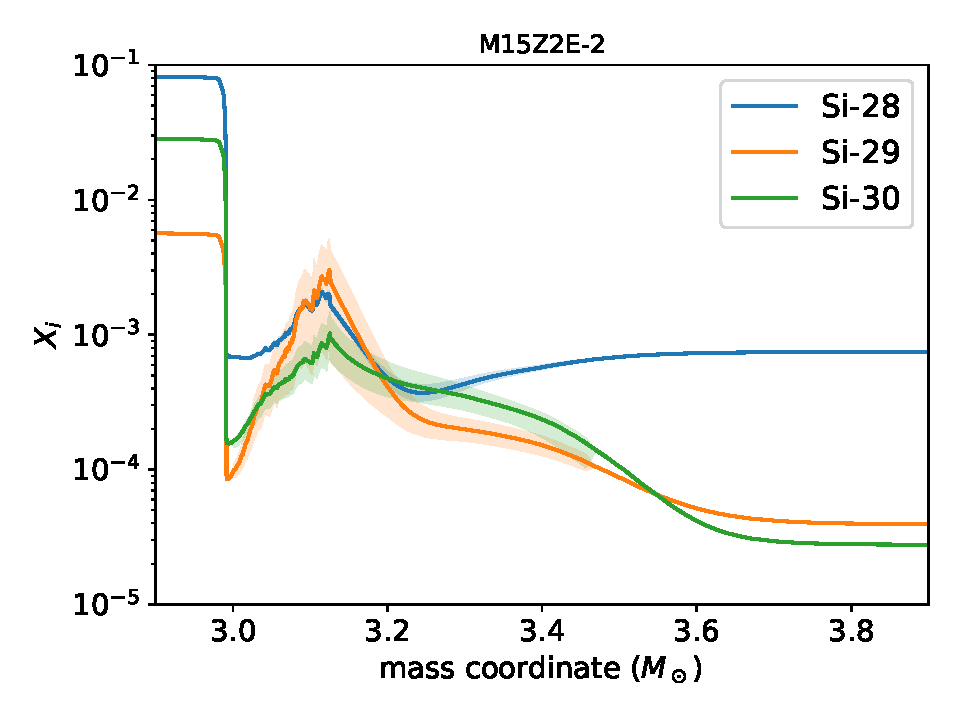
\includegraphics[width = \textwidth]{figs/M15Z2E-2_mcresult.pdf}
        \end{figure}
    \end{minipage}
\end{frame}

% in our mc calculation, we found that the nuclear uncertainties does affect the nucleosynthesis of silicon in massive stars. in particular, silicon 29 and 30 abundances are affected by the nuclear uncertainties while silicon 28 abundances remain largely unchanged. the picture shows the isotopic compositions in one of the stellar models after the supernova explosion. the solid lines represent the default model and the shades represent the variations derived from the monte carlo calculation. here shows four similar plots but for all four of the stellar models we tested. using these result, we integrate across the whole mass coordinate range to determined the integrated stellar nucleosynthesis yields. 


\begin{frame}{Stellar Nucleosynthesis Yields}
    \begin{minipage}{5cm}
        \begin{itemize}
            \setlength\itemsep{2em}
            \item Nuclear uncertainties have largest effect on \iso{29}{Si} yield at the order of 1-10\%
            \item Much smaller effects on \iso{28, \, 30}{Si} yields 
            % \item Variation factor: compared to default yield set given in \cite{Ritter_2018}
        \end{itemize}
    \end{minipage}
    \begin{minipage}{6.5cm}
    \centering
        \begin{figure}
            \centering
            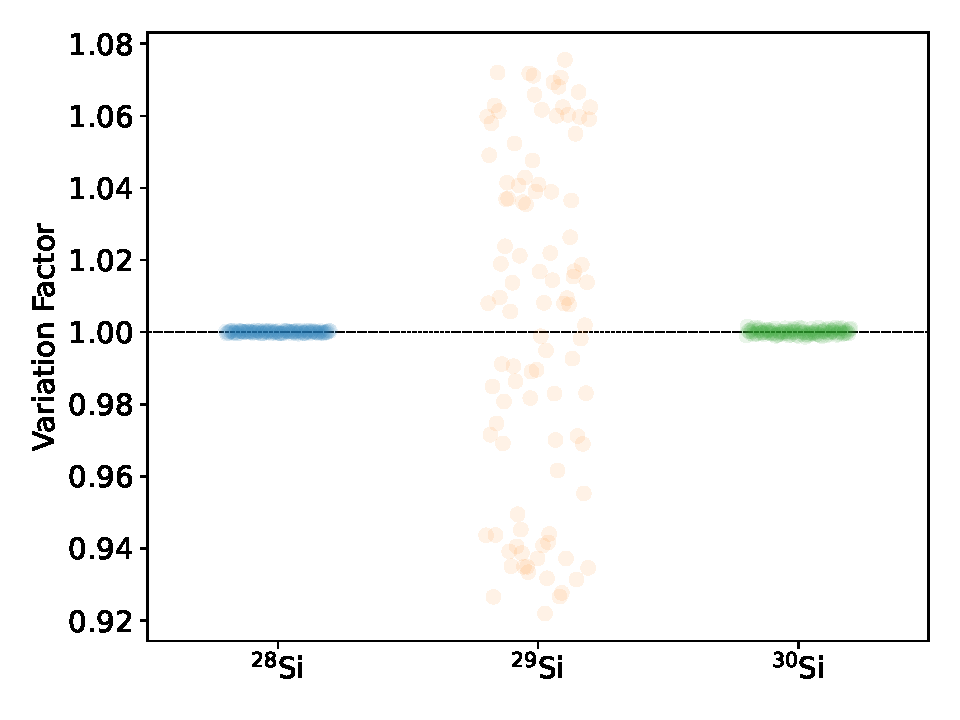
\includegraphics[width = \textwidth]{figs/M20Z1E-2_mcyieldresult.pdf}
        \end{figure}
    \end{minipage}
\end{frame}





\begin{frame}{Galactic Chemical Evolution of Silicon}
    \begin{minipage}{5.5cm}
        \begin{itemize}
        \setlength\itemsep{2em}
            \item Focus on 1.8-0.5 billion years prior to the formation of solar system
            \begin{itemize}
                \item From the formation time of the grain and the lifetime of their parent stars
            \end{itemize}
            \item \alert{Nuclear uncertainties do affect the GCE calculation  of silicon}
        \end{itemize}
    \end{minipage}
    \begin{minipage}{6cm}
    \centering
        \begin{figure}
            \centering
            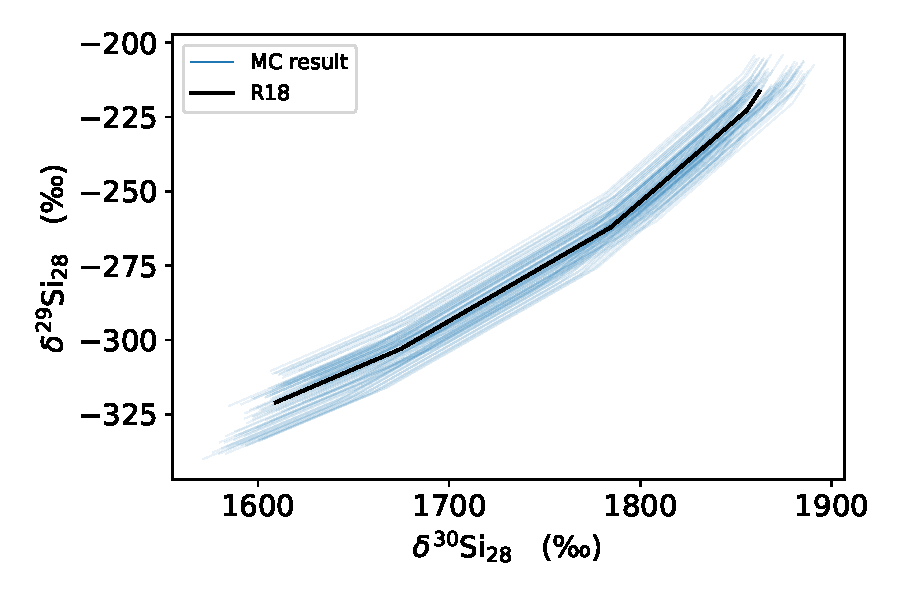
\includegraphics[width = \textwidth]{figs/GCE_2.pdf}
        \end{figure}
    \end{minipage}
    
\end{frame}

\begin{frame}{Comparison with SiC Mainstream Grains}
        \begin{minipage}{5.5cm}
        \begin{itemize}
            \item \alert{Nuclear uncertainties generate $\sim 5\%$ variation on the slope}

            \item Range of slope in our model: 0.42-0.40
            \begin{itemize}
                \item Smaller than mainstream line slope: 1.37 (\citealt{Zinner2007})
            \end{itemize}

            \item Discrepancy likely due to the effect of convective O-C shell merger
            % \begin{itemize}
            %     \item O-C shell merger in 1D models leads to overestimation of the production of \iso{30}{Si}
            % \end{itemize}
        
        \end{itemize}
    \end{minipage}
    \begin{minipage}{5.8cm}
    \centering
        \begin{figure}
            \centering
            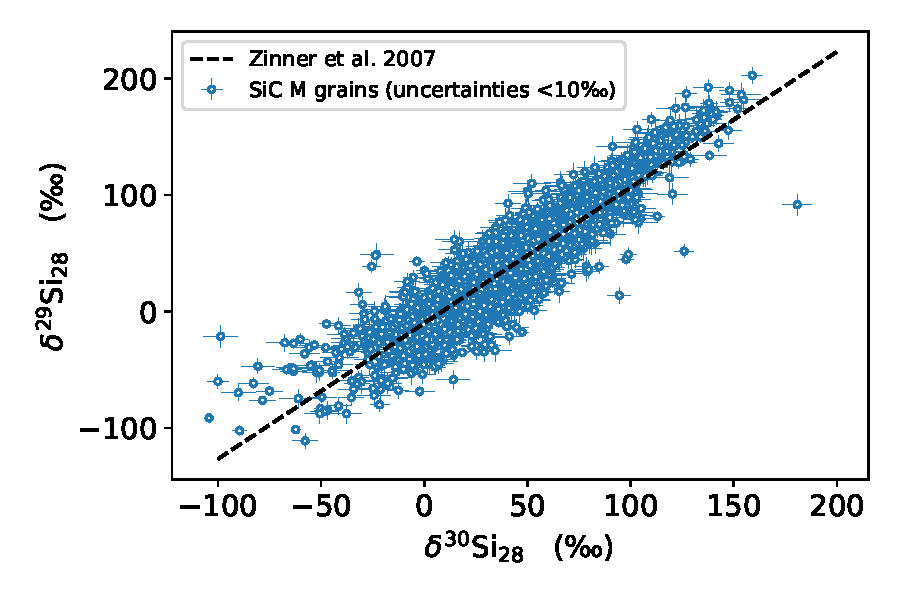
\includegraphics[width = \textwidth]{figs/stardust.pdf}
        \end{figure}
    \end{minipage}
\end{frame}


\begin{frame}{Summary and Conclusions}
        \begin{center}
            \textbf{First study to quantify the effect of nuclear uncertainties \\on the GCE of isotopes}
        \end{center}
        \begin{itemize}
        \setlength\itemsep{2em}
            \item Si isotopes are produced during explosive oxygen burning in massive stars
            \item Nuclear uncertainties affect stellar nucleosynthesis calculations of Si isotopes
            \item Nuclear uncertainties can lead to a $\sim5\%$ variation in the slope
            % \item Further investigation on the effects of O-C shell merger is needed
        \end{itemize}

\end{frame}

\begin{frame}{Further Studies}
    \begin{itemize}
    \setlength\itemsep{2em}
        \item Estimate the effects of O-C shell mergers
        \item Extend to a wider range of progenitor masses and initial metallicities 
        \item Investigate the effect when different sets of experimental rates are used
        
    \end{itemize}
\end{frame}

\begin{frame}{Acknowledgement}

\begin{itemize}
\setlength\itemsep{2em}
    \item Professor Reto Trappitsch and Professor James Cho
    \item Dr. Marco Pignatari, Dr. Benoit Cote
    \item NuGrid Collaboration
\end{itemize}
\end{frame}



\bibliography{ref}


\begin{frame}{Silicon carbide grains}
\begin{minipage}{5.5cm}
\begin{itemize}
    \item One of the best studied phases of stardust
    \item Classified and associated with various nucleosynthetic sources based on isotopic compositions
    \item Example: Mainstream grains come from AGB stars
    % \item $\delta$-value: deviation of isotope ratio from the average value of solar system (in $\permil$)
    \item $\delta$-notation:
       $\delta(^iX_j) =\left[\frac{\left(\frac{^iX}{^jX}\right)_{\text{sample}}}{\left(\frac{^iX}{^jX}\right)_{\odot}}-1\right] \times 1000$
    
\end{itemize}


\end{minipage}
    \begin{minipage}{6cm}
    \centering
        \includegraphics<1>[width = \textwidth]{figs/sic_n_c_all.pdf}
        \includegraphics<2>[width = \textwidth]{figs/sic_si_3iso_all.pdf}
    \end{minipage}
    
    %%%%%%%%%%%
    % The specific type of grains we are interested in is the silicon carbide grains and it is one of the best studied stardust grains. We can classify them based on their isotopic composition. Also, we can associate their isotopic composition with their nucleosynthetic source. The plot here shows the distribution of different types of grains in their nitrogen and carbon isotopic composition. 
    
    % the green box is the distribution found in the solar system. we can see that the isotopic compositions found in the grains are very different from solar 
    
    % here shows the distribution in the silicon isotopic composition. 
    % the axes: delta value
    % delta value: the deviation of isotope ratio from the average value of the solar system 
    % for example, in this plot, if the y value (the delta of 29/28) is negative, that means the sample is enriched in si28 or depleted in si29 compare to solar 

\end{frame}

\begin{frame}{Silicon produced in explosive oxygen burning}
    \begin{figure}
        \begin{subfigure}[b]{0.38\textwidth}
            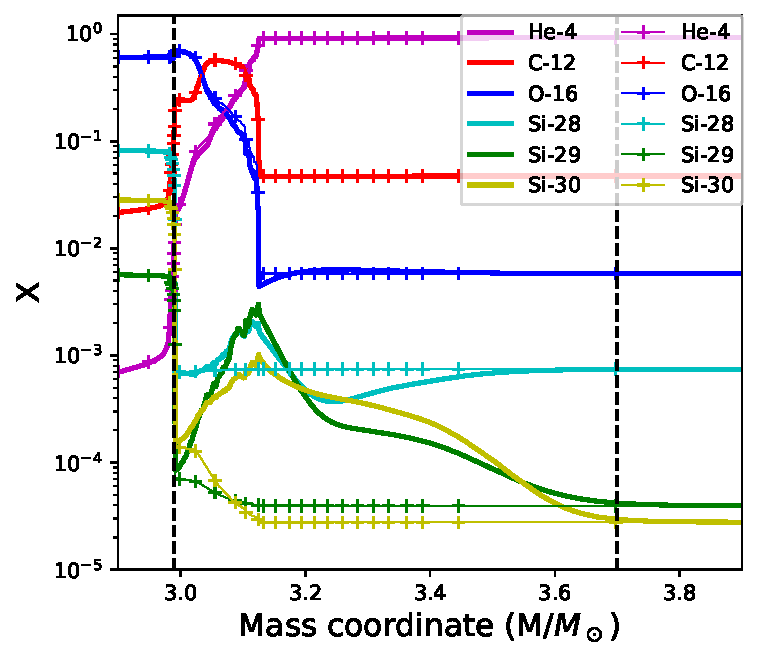
\includegraphics[width=\textwidth]{figs/150.02.pdf}
        \end{subfigure}
        \begin{subfigure}[b]{0.38\textwidth}
            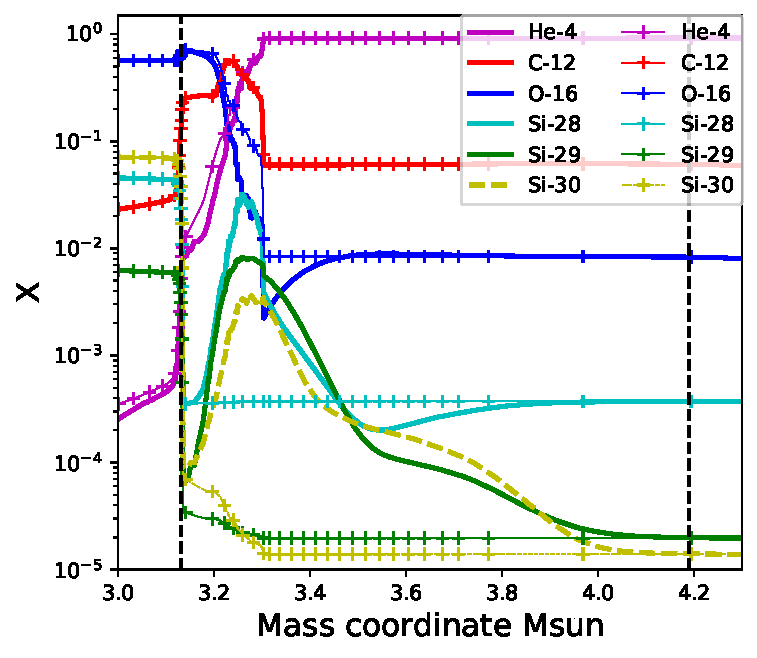
\includegraphics[width=\textwidth]{figs/150.01.pdf}
        \end{subfigure}
        
        \begin{subfigure}[b]{0.38\textwidth}
            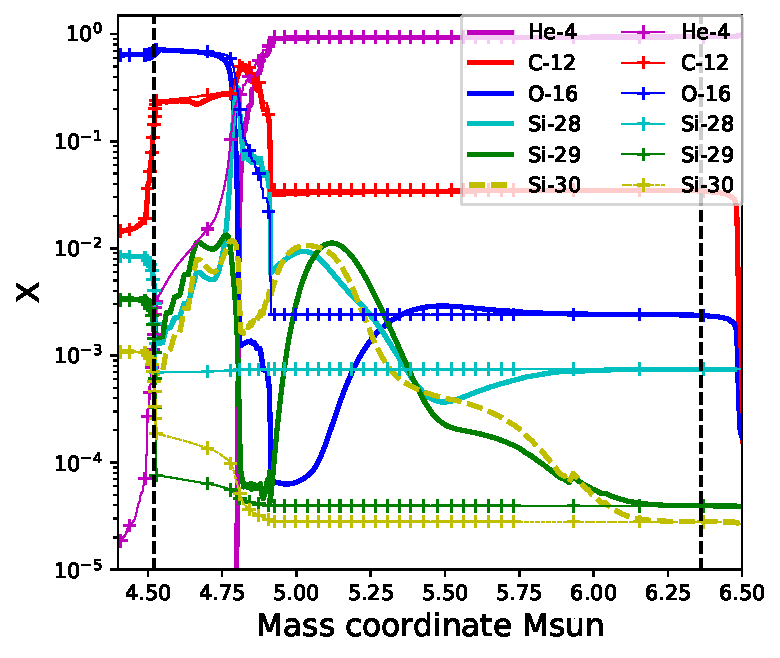
\includegraphics[width=\textwidth]{figs/200.02.pdf}
        \end{subfigure}
        \begin{subfigure}[b]{0.38\textwidth}
            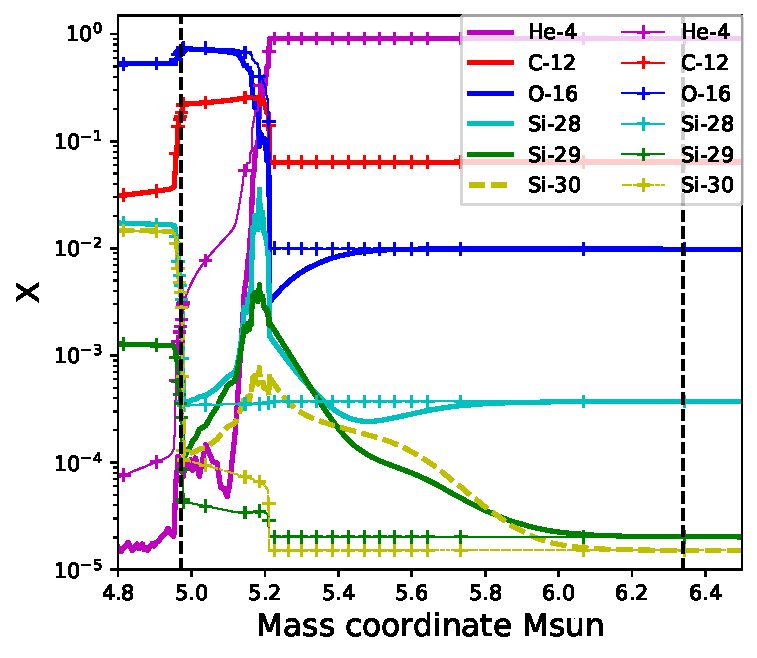
\includegraphics[width=\textwidth]{figs/200.01.pdf}
        \end{subfigure}
    \end{figure}
    
    % we have focesed on the explosive 
\end{frame}


\begin{frame}{Nuclear uncertainties affect nucleosynthesis of silicon in stars}
        \begin{figure}
        \begin{subfigure}[b]{0.42\textwidth}
            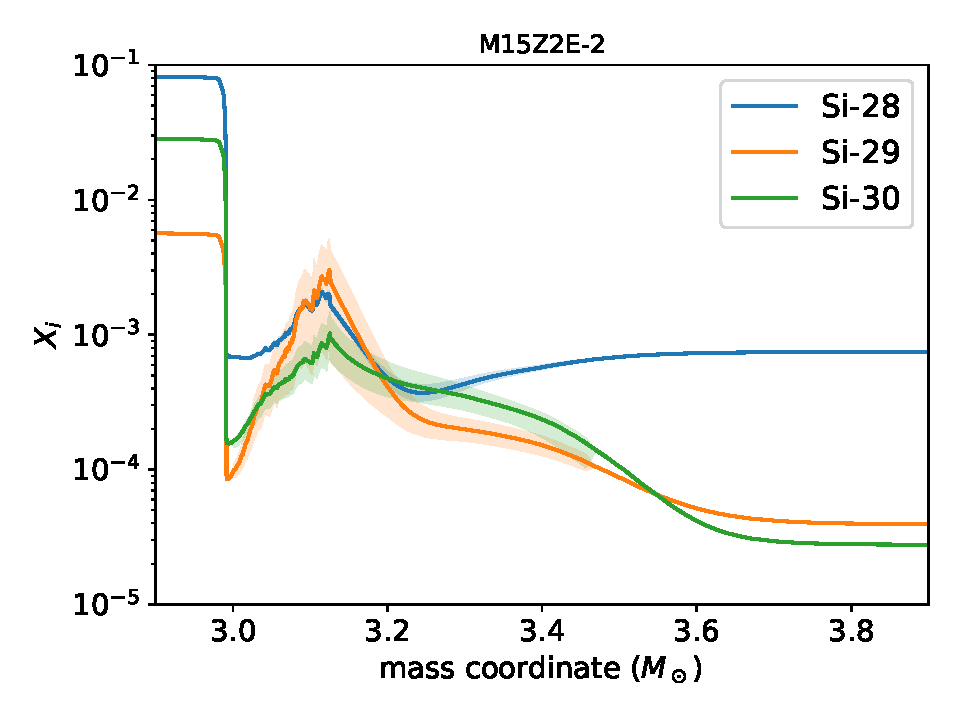
\includegraphics[width=\textwidth]{figs/M15Z2E-2_mcresult.pdf}
        \end{subfigure}
        \begin{subfigure}[b]{0.42\textwidth}
            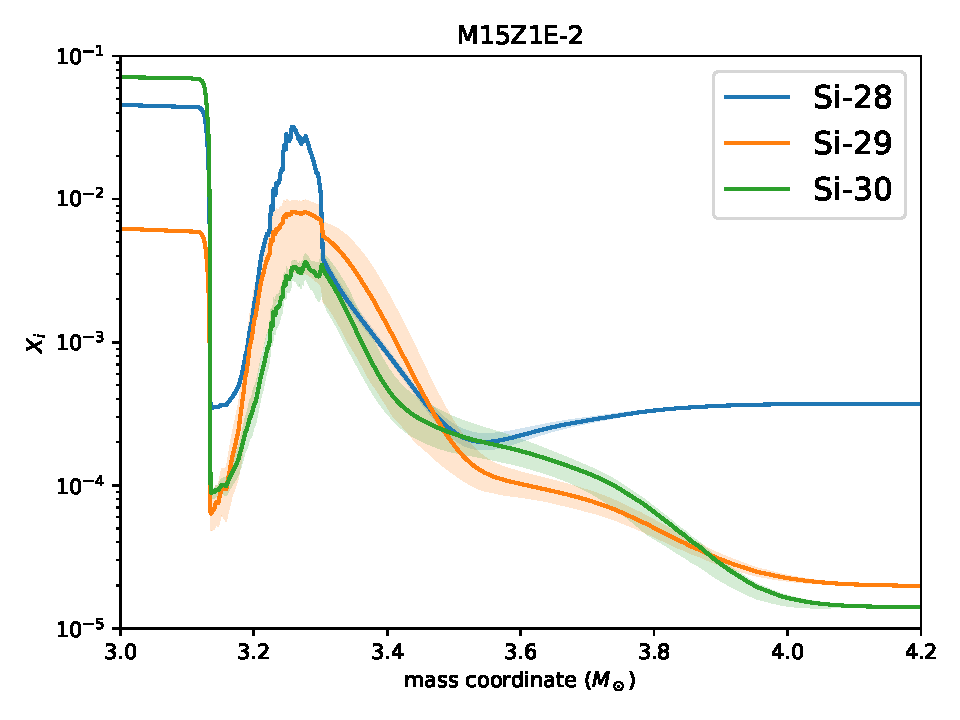
\includegraphics[width=\textwidth]{figs/M15Z1E-2_mcresult.pdf}
        \end{subfigure}
        
        \begin{subfigure}[b]{0.42\textwidth}
            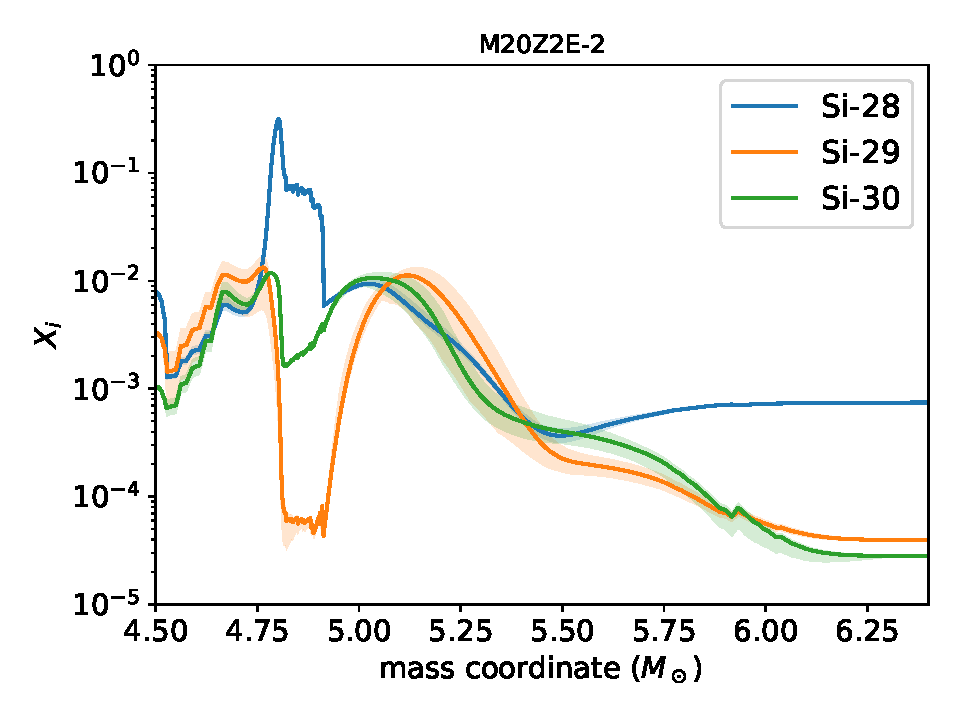
\includegraphics[width=\textwidth]{figs/M20Z2E-2_mcresult.pdf}
        \end{subfigure}
        \begin{subfigure}[b]{0.42\textwidth}
            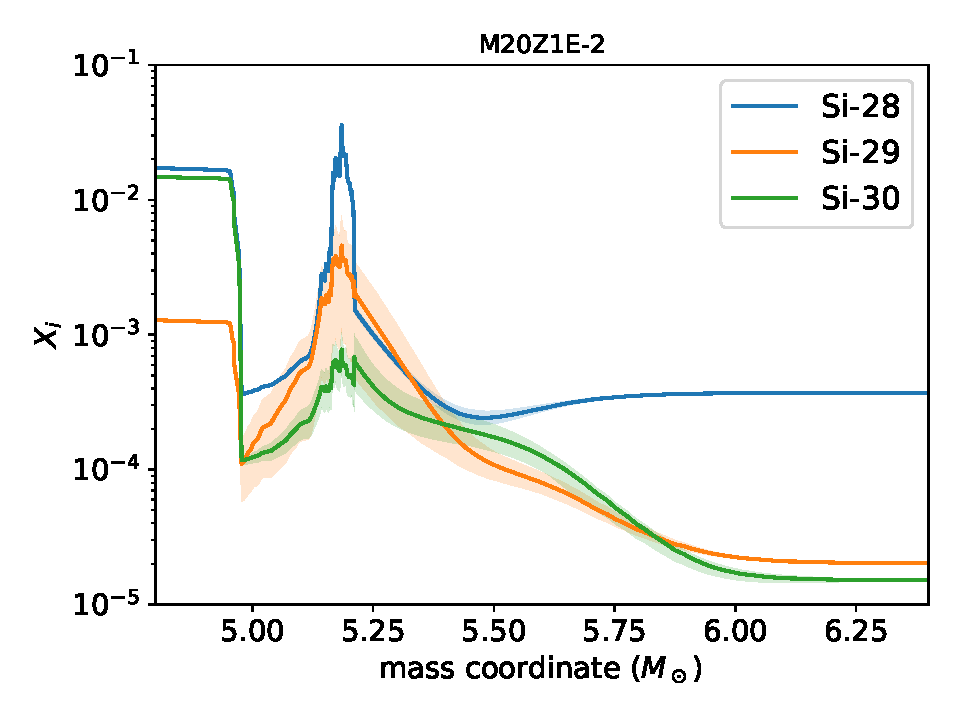
\includegraphics[width=\textwidth]{figs/M20Z1E-2_mcresult.pdf}
        \end{subfigure}
    \end{figure}
\end{frame}

\begin{frame}{Stellar nucleosynthesis yields}
        \begin{figure}
        \begin{subfigure}[b]{0.42\textwidth}
            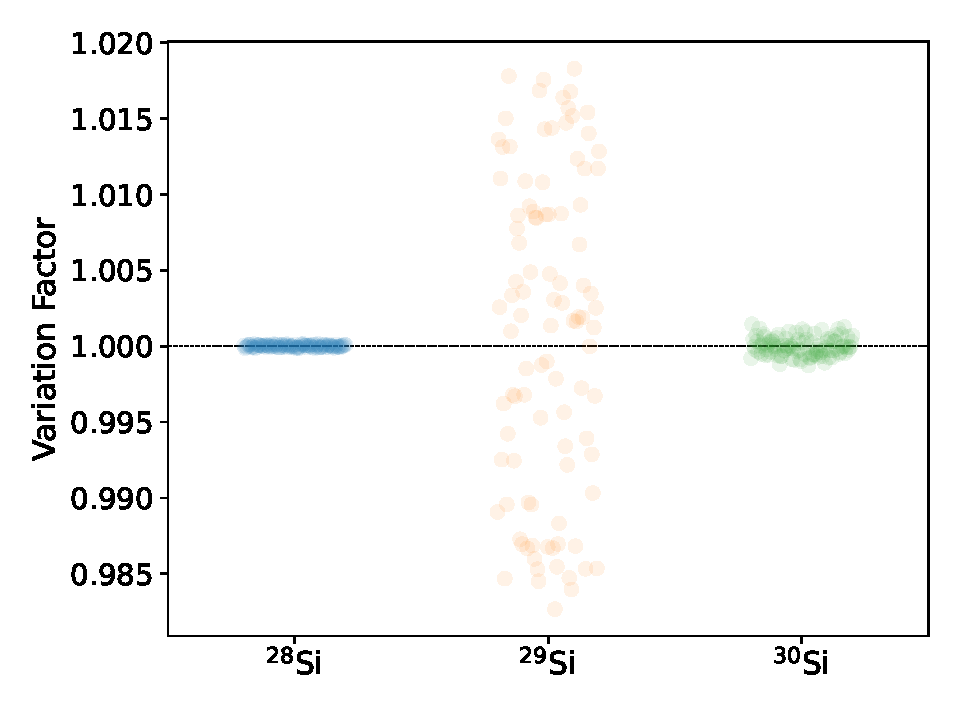
\includegraphics[width=\textwidth]{figs/M15Z2E-2_mcyieldresult.pdf}
        \end{subfigure}
        \begin{subfigure}[b]{0.42\textwidth}
            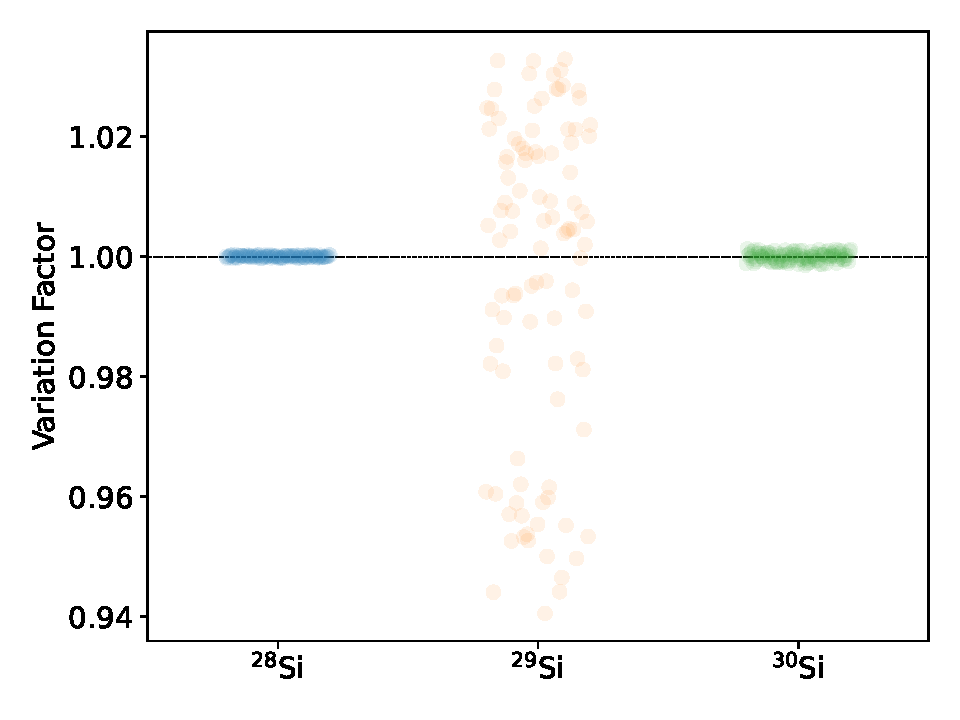
\includegraphics[width=\textwidth]{figs/M15Z1E-2_mcyieldresult.pdf}
        \end{subfigure}
        
        \begin{subfigure}[b]{0.42\textwidth}
            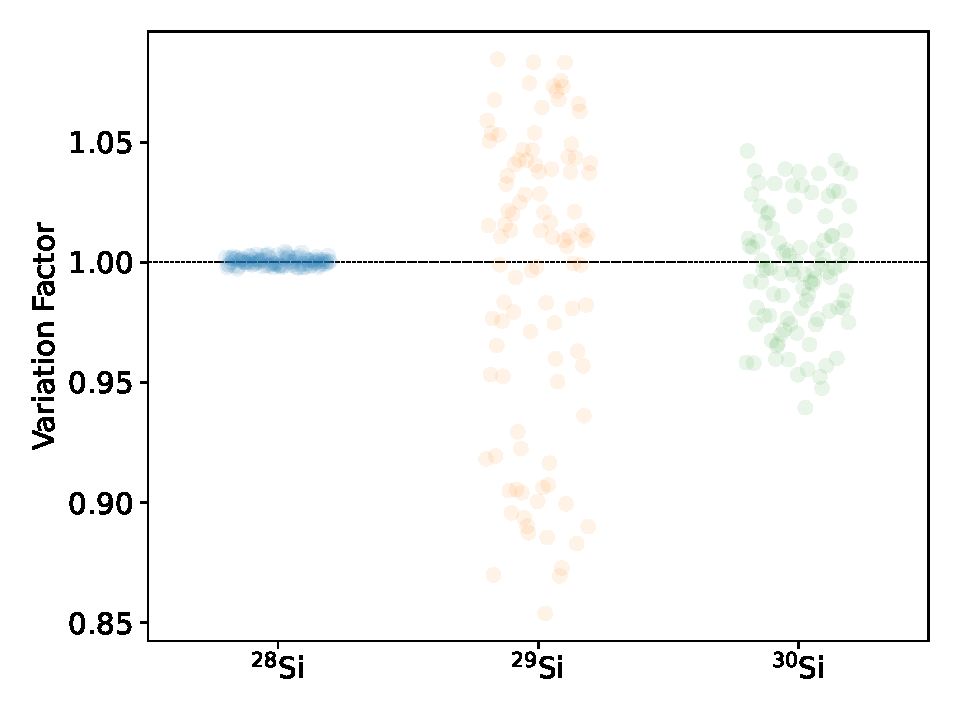
\includegraphics[width=\textwidth]{figs/M20Z2E-2_mcyieldresult.pdf}
        \end{subfigure}
        \begin{subfigure}[b]{0.42\textwidth}
            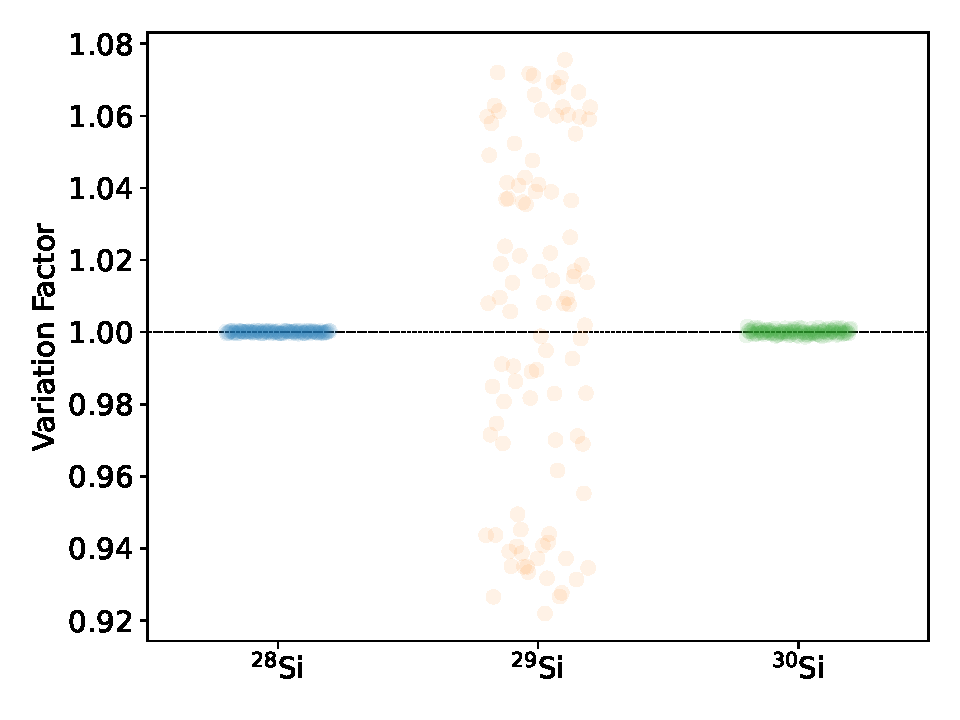
\includegraphics[width=\textwidth]{figs/M20Z1E-2_mcyieldresult.pdf}
        \end{subfigure}
    \end{figure}
\end{frame}

\end{document}